\documentclass[a4paper,12pt]{article} %{report}
\usepackage{graphicx}
\usepackage{booktabs}
\usepackage{hyperref}
\usepackage{longtable}
\usepackage{pdfpages} % http://mirror.unl.edu/ctan/macros/latex/contrib/pdfpages/pdfpages.pdf
\usepackage{natbib}
\usepackage{caption}
\captionsetup[table]{name=tabel}
\captionsetup[figure]{name=figuur}
\usepackage[utf8]{inputenc}
\usepackage[T1]{fontenc}
\usepackage{lmodern}
\usepackage{float}
\usepackage[export]{adjustbox}
\usepackage[none]{hyphenat}


\usepackage[colorinlistoftodos]{todonotes} % handig voor commentaar: gebruik \todo{}, zie ftp://ftp.fu-berlin.de/tex/CTAN/macros/latex/contrib/todonotes/todonotes.pdf

\renewcommand{\contentsname}{Inhoudsopgave}

\begin{document}


%%% DIT IS DE TITLE PAGE VOOR INFORMATIEKUNDE NIET VOOR AI OF INFORMATICA! 
%% GEBRUIK VOOR AI OF INFORMATICA JE EIGEN TITLEPAGE TEMPLATES\


\vspace{2.5cm}

% [CHANGE] The title of your thesis. If your thesis has a subtitle, then this
% should appear right below the main title, in a smaller font.
\begin{huge}
Title of the thesis
\end{huge}

\vspace{1.5cm}

% [CHANGE] Your full name. In case of multiple names, you can include their
% initials as well, e.g. "Jan G.J. van der Wegge".
N.T de Visscher\\
% [CHANGE] Your student ID, as this has been assigned to you by the UvA
% administration.
10667474

\vspace{1.5cm}

% [DO NOT CHANGE]
Bachelor thesis\\
% [CHANGE] Whether your Bachelor thesis is 6 ECTS (regular) or 9 ECTS (Honours
% programme).
Credits: 12 EC

\vspace{0.5cm}

% [DO NOT CHANGE] The name of the educational programme.
Bachelor Opleiding Informatiekunde

\vspace{0.25cm}

% [DO NOT CHANGE] The addess of the educational programme.
University of Amsterdam\\
Faculty of Science\\
Science Park 904\\
1098 XH Amsterdam

\vspace{4cm}

\emph{Supervisor}\\
% [CHANGE] The name of your supervisor. Include the titles of your supervisor,
% as well as the initials for *all* of his/her first names.
Dr. M. J. Marx

\vspace{0.25cm}

% [CHANGE] The address of the institute at which your supervisor is working.
% Be sure to include (1) institute (is appropriate), (2) faculty (if
% appropriate), (3) organisation name, (4) organisation address (2 lines).
ILPS, IvI\\
Faculty of Science\\
University of Amsterdam\\
Science Park 904\\
1098 XH  Amsterdam

\vspace{1.5cm}

% [CHANGE] The date at which you will finalize and submit your thesis.
2016-06-26

\newpage\cleardoublepage


\pagebreak

\tableofcontents

\pagebreak

\begin{abstract}
% [CHANGE] 
\end{abstract}


\pagebreak


% Here you input all your sections in seperate files

\section{Introduction}
\label{sec:intro}

Dit onderzoek is een replicatie-onderzoek aan de hand van een eerder uitgevoerd onderzoek dat als paper is gepubliceerd. Het paper in kwestie beschrijft een onderzoek naar de "State of the Union" speeches uit Amerika van~\cite{state}. In dat onderzoek werd gekeken naar wat er veranderde binnen de speeches sinds ze voor het eerst werden gehouden en hoe de speeches er hedendaags uitzien. Er werd gekeken naar de verschuiving in taalgebruik en inhoud in de speeches. Dit werd gedaan om een beeld te krijgen wat de belangrijke onderwerpen in een speech waren en welke thema's behandelt \todo{huh, zeker weten?} werden over de jaren. \todo{Zeg hier ook dat het om XX jaar gaat, van A tot B, en dat ze jaarlijks worden uitgesproken.}
\\
\todo{gebruik geen backslah backslah maar een lege regel voor een nieuwe paragraaf}
De State of the Union is niet de enige speech die al lange tijd wordt gehouden. Zo ook de troonredes van ons eigen Nederland. Deze troonredes worden sinds 1818 jaarlijks door de koning/koningin gegeven. De troonredes kunnen gezien worden als een Nederlandse versie van de State of the Union. De troonredes bevatten echter vaak reflecties op het afgelopen jaar in plaats van een update over de staat van het land \todo{Dit is geen nederlands, maar een erg lelijk anglicisme}. De staat van het land wordt ook wel besproken, maar meer in de context van de wereld, namelijk een kijk naar de positie van Nederland in de wereld. Dit is echter niet altijd het geval geweest. Zo was de inhoud vroeger anders dan nu, net als het taalgebruik.
\\
Tijdens het onderzoek zal er gekeken worden naar de veranderingen in de troonredes over de jaren. Het gaat hier vooral om de onderwerpen en thema's die behandeld worden. Er zal allereerst niet specifiek worden gekeken naar de verandering in taalgebruik en grammatica, maar dit kan wel gebruikt worden om een beeld te vormen over de veranderingen van de troonredes.
\\
Om het onderzoek een duidelijke richting te geven zal gepoogd worden de volgende onderzoeksvraag te beantwoorden:

\begin{itemize}
\item Hoe kan "word co-occurence" als tekstanalyse techniek worden gebruikt om de verschuiving in onderwerpen/thema's over 200 jaar troonredes weer te geven?
\end{itemize}

\begin{description}
\item[RQ1]  We   beantwoorden deze vraag met behulp van de volgende deelvragen:
\begin{enumerate}
\item Wat is "word co-occurence" en hoe worden deze uit teksten verzameld? Evaluatie sectie~\ref{sec:eva}.
\item Hoe kan betekenis worden gegeven aan co-occurences?
\item Hoe wordt de context van de tekst in acht gehouden?
\item Wat voor invloed heeft de verandering van taal(gebruik) over de jaren op de analyse technieken?
\end{enumerate}
\end{description}
\todo{Ik zou dan je deelvragen ook nummeren. De eerste deelvraag is geen vraag die je hier moet stellen. Ik zou ook wat technische vragen opnemen. je kunt ok beginnen met "Zijn de methoden die zijn ontwikkeld in \cite{state} 1) toepasbaar op het Nederlandse troonrede corpus en 2) leveren ze ook inzichtelijke resultaten op?. \\
Dan kun je daarbij per techniek een deelvraag stellen: is het mogelijk het voor het NL te doen? En wat levert het op? Je kunt dan heel simpel vertellen dat inderdaad POS tagging prima werkt voor het NL, maar dat ie foutjes maakt, etc, etc\\
Zulke vragen en deelvragen geven jou en de lezer meer richting en alles wordt er makkelijker door.}


\paragraph{Overview of thesis}
Hier geef je even kort weer wat in elke sectie staat.\newpage\cleardoublepage
\section{Related Work}
\label{sec:rel}

Deze sectie bestaat uit een aantal "blokken", waarin je per blok de relevante literatuur beschrijft. 

Neem alleen literatuur op die van belang is voor jouw onderzoeksvraag en deelvragen.

Typisch heb je 1 blok voor je hoofdvraag en per deelvraag \textbf{RQi} een blok. 


\subsection{RQ1}

\subsection{RQ2}\newpage\cleardoublepage
\section{Methodology}
\label{sec:meth}


\subsection{Description of the data}
De dataset die gebruikt gaat worden om deze vragen te beantwoorden is een verzameling van troonredes sinds 1814. Deze troonredes zijn terug te vinden op www.troonredes.nl~\citep{troonredes} . Om een duidelijker beeld te geven van wat de troonrede nu precies is eerst een kleine introductie van wat de troonredes nu precies zijn. 
\\
De troonrede wordt jaarlijks door de koning(in) uitgesproken op Prinsjesdag. De eerste troonrede werd in 1818 als een algehele toespraak voor de Staten-generaal gehouden. De troonredes worden vooral gebruikt om wets- en beleidsveranderingen
door te geven en als beschouwing op het afgelopen jaar en de staat van het land. In recentere jaren heeft deze beschouwing zich ook uitgebreid naar gebeurtenissen door de hele wereld die invloed uitoefenen op de Nederlandse staat. Sinds 1848 worden de troonredes geschreven door ministers en is het kabinet verantwoordelijk voor de uitspraken. Dit zorgt ervoor dat de troonredes een beeld geven van wat de Nederlandse regering op dat moment belangrijk vindt.
\subsection{Missing data}
Er zijn verscheidene jaren waarvan er geen data beschikbaar is, dit doordat er niet elk jaar een troonrede gegeven is. Dit heeft verschillende redenen, zoals oorlogen, angst voor rellen, onvrede over het kabinet of gezondheidsredenen omtrent de koning(in). Dit zorgt ervoor dat niet elk jaar sinds 1818 wordt gerepresenteerd door een troonrede. Omdat de inhoud van de troonredes worden als
verzamelde dataset wordt gebruikt heeft dit minimaal invloed op de uiteindelijke uitkomsten van het onderzoek dat er jaren missen. Door de missende jaren is het weergeven van de verschuiving in onderwerpen mogelijk niet volledig representatief, omdat er geen uitspraken gedaan kunnen worden over de missende jaren.


\subsection{Quality of the data}
Hier moet nog een deel komen over het feit of het ingescand is of ingetypt.

\pagebreak
\subsection{Wat plotjes en tabelletjes}

Zie het IPython Notebook voor de code om vanuit pandas een poltje op te slaan en een dataframe als tabel op te slaan. Het werkt ideaal! 

De interrupties van Wilders staan beschreven in Figure~\ref{fig:wilders} en Tabel~~\ref{tab:Wilders}.



%\begin{figure}
%\begin{center}
%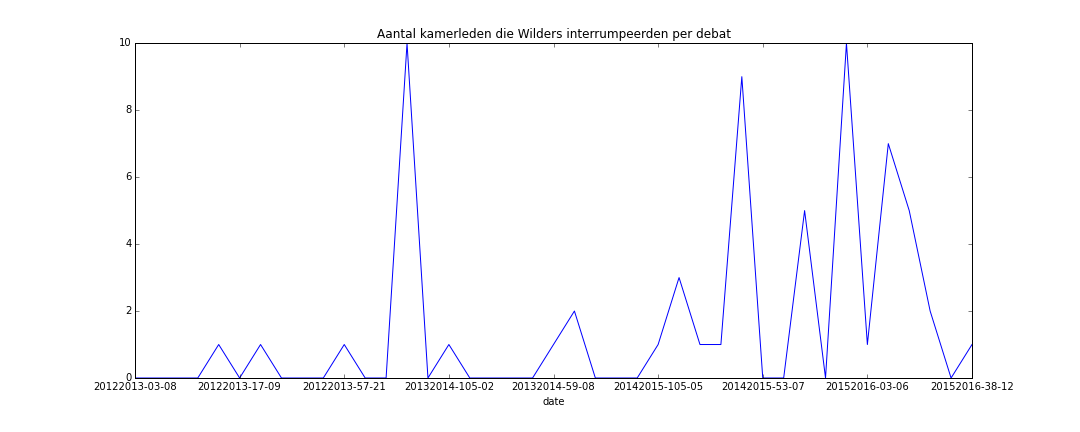
\includegraphics[width=\linewidth]{fig/WildersPlot.png}
%\caption{\label{fig:wilders} Aantal interrupties van Wilders in de Tweede Kamer door de tijd (periode 2012-2016).}
%\end{center}
%\end{figure}


\pagebreak

%\begin{table}[h]
%\begin{footnotesize}
%\begin{tabular}{lrl}
\toprule
{} &  indegree &                               interruptie\_volgorde \\
date            &           &                                                    \\
\midrule
20122013-03-08  &         0 &                                                    \\
20122013-07-16  &         0 &                                                    \\
20122013-100-03 &         0 &                                                    \\
20122013-100-06 &         0 &                                                    \\
20122013-17-06  &         1 &                         Pechtold-Pechtold-Pechtold \\
20122013-17-09  &         0 &                                                    \\
20122013-21-04  &         1 &                         Pechtold-Pechtold-Pechtold \\
20122013-22-08  &         0 &                                                    \\
20122013-32-06  &         0 &                                                    \\
20122013-48-23  &         0 &                                                    \\
20122013-57-21  &         1 &  Pechtold-Pechtold-Pechtold-Pechtold-Pechtold-P... \\
20122013-76-03  &         0 &                                                    \\
20122013-76-06  &         0 &                                                    \\
20132014-05-02  &        10 &  Roemer-Roemer-Van Haersma Buma-Van Haersma Bum... \\
20132014-06-04  &         0 &                                                    \\
20132014-105-02 &         1 &  Pechtold-Pechtold-Pechtold-Pechtold-Pechtold-P... \\
20132014-105-06 &         0 &                                                    \\
20132014-14-03  &         0 &                                                    \\
20132014-14-06  &         0 &                                                    \\
20132014-52-18  &         0 &                                                    \\
20132014-59-08  &         1 &                               Klaver-Klaver-Klaver \\
20142015-02-08  &         2 &  Pechtold-Pechtold-Pechtold-Pechtold-Pechtold-P... \\
20142015-03-06  &         0 &                                                    \\
20142015-09-09  &         0 &                                                    \\
20142015-100-05 &         0 &                                                    \\
20142015-105-05 &         1 &                                  Pechtold-Pechtold \\
20142015-111-04 &         3 &  Pechtold-Pechtold-Pechtold-Pechtold-Pechtold-P... \\
20142015-111-07 &         1 &                                  Pechtold-Pechtold \\
20142015-39-71  &         1 &                                  Pechtold-Pechtold \\
20142015-41-07  &         9 &  Samsom-Samsom-Pechtold-Pechtold-Pechtold-Kuzu-... \\
20142015-53-07  &         0 &                                                    \\
20142015-61-23  &         0 &                                                    \\
20142015-79-07  &         5 &  Klaver-Klaver-Klaver-Gesthuizen-Gesthuizen-Ges... \\
20142015-95-06  &         0 &                                                    \\
20152016-02-07  &        10 &  Pechtold-Pechtold-Pechtold-Pechtold-Slob-Slob-... \\
20152016-03-06  &         1 &       Pechtold-Pechtold-Pechtold-Pechtold-Pechtold \\
20152016-14-02  &         7 &  Klaver-Klaver-Roemer-Roemer-Roemer-Roemer-Sams... \\
20152016-14-05  &         5 &  Van Haersma Buma-Van Haersma Buma-Van Haersma ... \\
20152016-27-03  &         2 &  Segers-Segers-Segers-Segers-Kuzu-Kuzu-Kuzu-Kuz... \\
20152016-38-10  &         0 &                                                    \\
20152016-38-12  &         1 &                                        Klein-Klein \\
\bottomrule
\end{tabular}

%\end{footnotesize}
%\caption{\label{tab:Wilders} Door wie werd Wilders onderbroken en hoe vaak per debat.}
%\end{table}


\pagebreak
\subsection{Methods}
Het gehele corpus bestaat uit 117 verschillende troonredes, welke in totaal uit 143875 woorden bestaan. Om uit deze data te kunnen achterhalen of er overkoepelende thema's/onderwerpen zijn en wat deze mogelijk zijn wordt er gebruik gemaakt van tekstanalyse technieken. Specifiek wordt er gebruik gemaakt van co-occurence aanpakken.~\cite{callon1991co} Hierbij worden categoriën geinduceerd door te kijken naar het samen voorkomen van termen in afzonderlijke stukken tekst. Hierbij is het doel om uit te vinden welke termen relevant zijn en hoe deze zich over tijd met andere termen associëren. Met behulp van deze informatie zouden er uitspraken gedaan kunnen worden over de onderwerpen die termen impliceren. Hiermee kunnen dan uitspraken worden gedaan over de inhoud van een specifieke troonrede aan de hand van de termen in de tekst. 
\\
Voordat deze uitspraken echter kunnen worden gedaan moet de data eerst worden verwerkt zodat er analyse op kan worden gedaan. Hiervoor worden de teksten van de troonredes eerst gelemmatiseerd. Hierdoor worden de woorden herleid tot hun lemma(stam), waardoor ze kunnen worden geanalyseerd als één term. Met behulp van deze gelemmatiseerde termen wordt een co-occurence matrix opgesteld. Deze matrix omvat voor alle combinaties van termen de frequentie dat ze samen in een paragraaf voorkomen. 
\\
Voor alle combinaties uit deze matrix wordt een nabijheidsscore berekend via het volgende algoritme. $$S(W_1,W_2)=\frac{\sum_{c\epsilon W\{W_1,W_2\},I(W_1,c)>0}min(I(W_1,c),I(W_2,c))}{\sum_{c\epsilon W\{W_1,W_2\},I(W_1,c)>0}I(W_1,c)}$$ Dit algoritme maakt gebruik van de woorden uit het gehele corpus om context te bepalen. Hiervoor wordt voor elke combinatie woorden (W1,W2) gekeken naar de woorden waarmee ze
samen in een paragraaf voorkomen. De som van I(W,C) voor alle woorden (C) uit het corpus waarvoor geldt dat I(W,C) > 0 wordt voor beide woorden berekend. Als hieruit volgt dat I(W,C) voor beide woorden gelijk is kan men stellen dat als W1 in een paragraaf voorkomt W2 ook voorkomt en vice versa. Een verwantschapsscore van 0 geeft aan dat de woorden nooit samen in een paragraaf voorkomen. Aan de hand van deze score wordt een gewogen semantisch netwerk gevormd met de termen als nodes en de gewichten op de edges. Om de termen binnen dit netwerk te kunnen analyseren wordt gebruik gemaakt van een community detectie algoritme. Het specifieke algoritme dat gebruikt wordt is dat van~\cite{blondel2008fast}. Het doel van dit algoritme is om vanuit het gewogen netwerk clusters te vormen van samenhangende subsets van termen. Afhankelijk van de termen binnen deze
clusters kunnen deze clusters gezien worden als indicatief voor onderwerpen/thema's binnen het corpus. Dit induceren van onderwerpen moet een overzicht geven van de verschillende termen die tot  een onderwerp behoren en hoe sterk de samenhang is tussen termen binnen een onderwerp. Ook zou het een beeld moeten geven van de samenhang tussen verschillende onderwerpen. 
\\
Om tot het gewogen netwerk te komen dat gebruikt kan worden voor de clustering wordt de dataset van woorden binnen het gehele corpus eerst gereduceerd tot de meest relevante data. Allereerst wordt de dataset gelemmatiseerd, waarna de 1000 meest voorkomende termen gebruikt worden om de co-occurence matrix op te stellen. De nabijheidsscore voor de termen uit deze matrix worden berekend en om ervoor te zorgen dat enkel de meest relevante termen worden meegegeven aan het community detectie algoritme wordt een drempel bepaald. Deze drempel geeft aan vanaf welke waarde van de nabijheidsscore de co-occurence combinaties door het algoritme verwerkt worden. De drempelwaarde ligt tussen de 0 en 1 en wordt bepaald door vanaf 0 de score telkens op te hogen. De drempelwaarde is bereikt als er binnen het netwerk een component van meer dan 2 nodes verdwijnt. Hiermee worden de zwak verbonden nodes uit het netwerk verwijderd. De drempelwaarde die gevonden is voor ons netwerk is θ=0.65. Het resulterende netwerk is door het community detectie algoritme verwerkt om de verschillende subsets te kunnen identificeren. Vanuit deze subsets wordt bepaald aan de hand van de termen die er onder vallen of er een onderwerp mee geassocieerd kan worden.


\subsubsection{RQ1}

\subsubsection{RQ2}\newpage\cleardoublepage
\section{Evaluation}
\label{sec:eva}

Met een subsectie voor elke deelvraag.

In hoeverre is je vraag beantwoord?

Een mooie graphic/visualisatie is hier heel gewenst.

Hou het kort maar krachtig.

\subsection{Zijn de methodes gebruikt in \cite{state} toepasbaar op het Nederlandse troonrede corpus?}

De Nederlandse troonrede is net zoals het de Amerikaanse State of the Union een toespraak die jaarlijks vanuit de overheid worden gegeven. In beide gevallen wordt de voordracht door één positie voorgedragen, voor Nederland is dit de koning(in) en voor de VS is dit de president. Voor beide teksten geldt dat ze zijn opgebouwd uit verschillende paragrafen en er veelal voor elke paragraaf één onderwerp centraal staat. Beide hebben een centraal motief gericht op het meedelen van de huidige staat van het land en mogelijk voornemens voor het komende jaar. 
Omdat de opbouw en het doel van beide teksten zoveel op elkaar lijken zijn de methodes die gebruikt zijn binnen \cite{state} goed toepasbaar op het corpus van de Nederlandse troonredes. Hierbij hoeven er maar kleine aanpassingen gemaakt te worden, waarbij het grootste verschil ligt in het feit dat de teksten in verschillende talen zijn geschreven. Voor het Nederlands betekent gaf dit enkele problemen omdat woorden over de jaren op verschillende manieren zijn geschreven en de taal over de jaren is verandert. Zo werd het woord "de" vroeger als "den" geschreven. Hierdoor zijn enkele woorden die vroeger anders geschreven werden niet opgevangen door de POS-tagging. Op het moment dat dit duidelijk werd is het handmatig aangepast. Op deze manier is er net als in \cite{state} het corpus gereduceerd tot de relevante zelfstandige naamwoorden. Hierbij is dus gebruik gemaakt van modules die op de Nederlandse taal getraind waren. Hierna zijn de 1000 meest voorkomende termen gebruikt worden om de co-occurence matrix op te stellen dat gebruikt is om de nabijheidsscore te berekenen waarmee het semantische netwerk is gevormd.

\subsection{Zijn de resultaten representatief voor de werkelijkheid?}

De verkregen resultaten zijn de geïnduceerde onderwerpen en het daarmee verkregen overzicht van onderwerp verschuivingen. Hiervoor was het belangrijkste dat er vanuit het semantische netwerk door middel van het community clustering algoritme duidelijke clusters gevormd werden. Vanuit de termen binnen een cluster kan een achterliggend onderwerp worden bepaald dat door deze termen wordt geïmpliceerd. Het is dus noodzakelijk dat de clusters duidelijk verschillend van elkaar zijn en de relatie tussen de termen in een cluster zo min mogelijk verschillende onderwerpen impliceren. Hoe duidelijker de relatie is tussen de termen in een cluster hoe makkelijker het is om er een onderwerp aan te koppelen. Dit is het makkelijkst voor clusters die gecentreerd zijn rondom één term, zoals "onderwijs" of "ontwikkeling". 

De onderwerpen die gevonden zijn staan in tabel \ref{onderwerpen}:
\begin{table}[htb]
\centering
\begin{tabular}{ll}
\toprule
{} &                Onderwerpen \\
\midrule
 &  regeringsbeleid \\
 &        onderwijs \\
 &    arbeidsbeleid \\
 &  koloniaalbeleid \\
 &        wetgeving \\
 &     ontwikkeling \\
 &    staatplanning \\
 &         defensie \\
\bottomrule
\end{tabular}
\caption{Geïmpliceerde onderwerpen}
\label{onderwerpen}
\end{table}

Voor elk onderwerp is er een lijst met termen waarvoor geldt dat als deze voorkomen in een tekst ze dat onderwerp impliceren. Aan de hand van deze lijst is een grafiek opgesteld met daarin voor elk jaar de hoeveelheid dat een onderwerp besproken werd. Dit is gedaan door te kijken naar de volledige tekst van dat jaar en voor elk woord na te gaan bij welk onderwerp het hoort. Hierna is door gebruik te maken van een normaal verdeling een grafiek gevormd die per onderwerp procentueel aangeeft hoeveel van de troonrede besteed was aan de behandeling van dat onderwerp. Hieruit volgt de grafiek in figuur \ref{onderwerpverdeling}:

\begin{figure}[H]
\hfill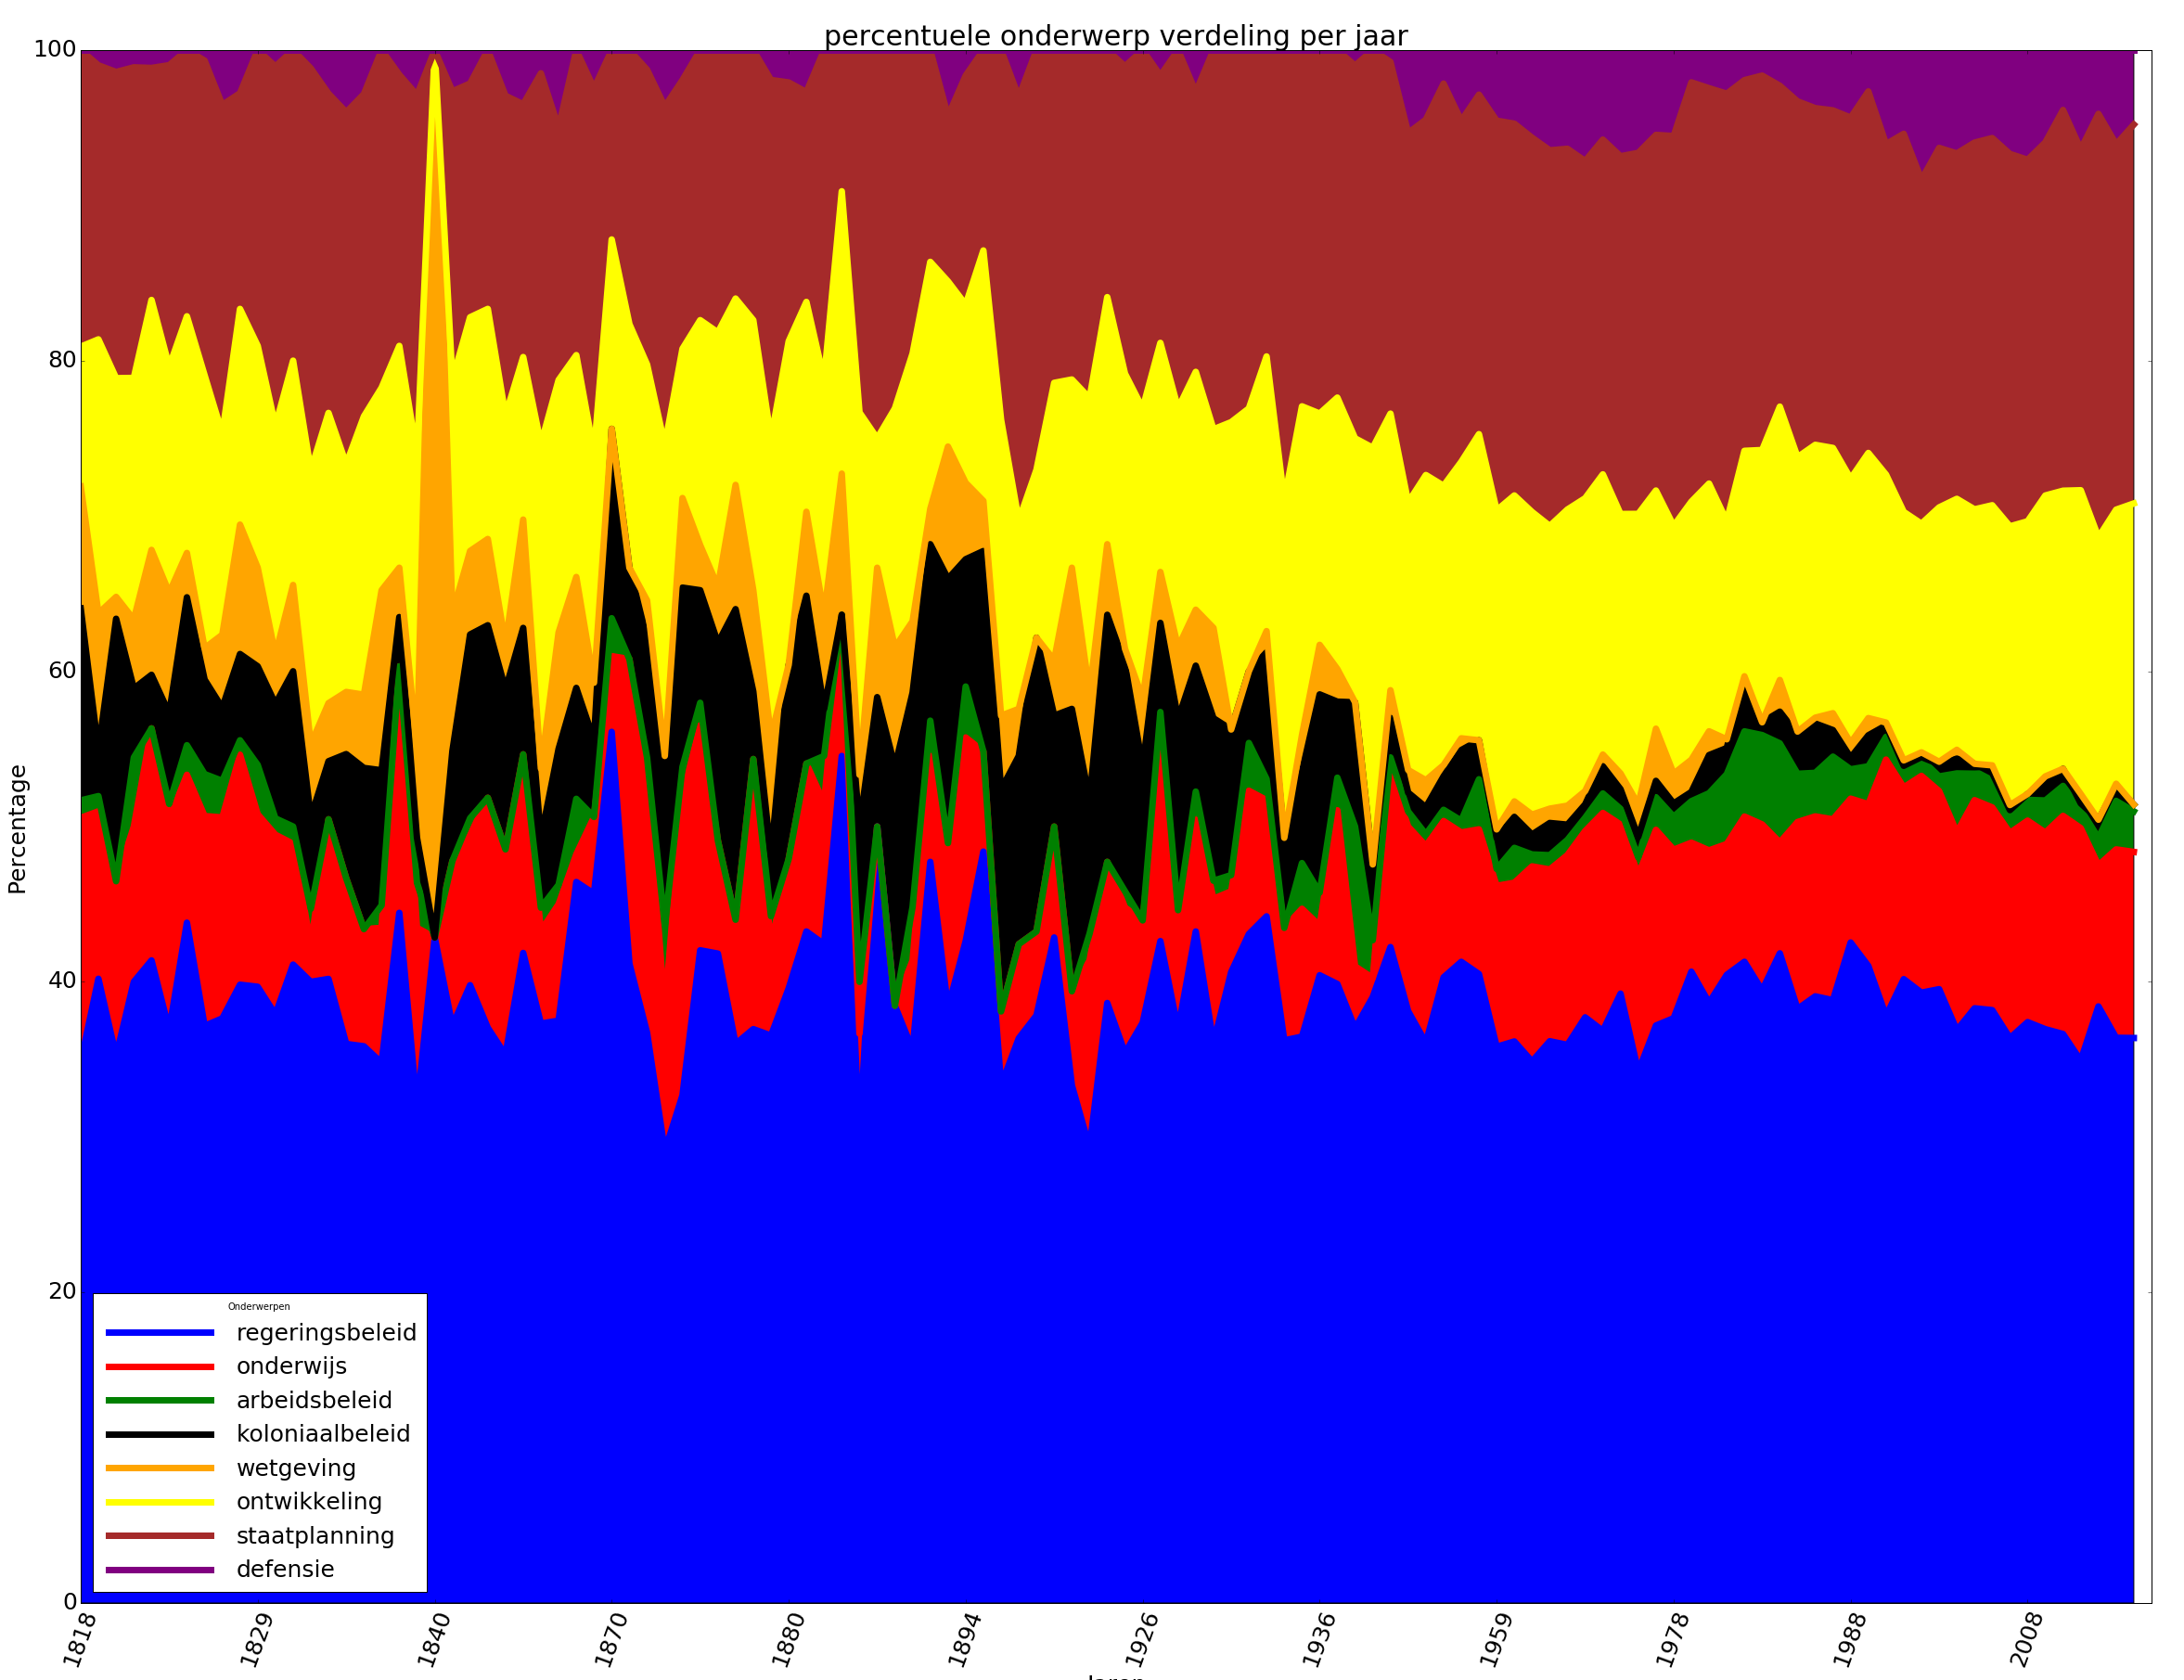
\includegraphics[width=1.2\textwidth,left]{fig/onderwerpverdeling}
\caption{\label{onderwerpverdeling} Verschuiving van inhoud van troonredes over de jaren aan de hand van de gevonden onderwerpen.}
\end{figure}


Vanuit deze grafiek is duidelijk af te lezen welke onderwerpen het belangrijkst waren in een jaar. Zo is bijvoorbeeld duidelijk te zien dat er rond 1839-40 het onderwerp wetgeving sterk naar voren komt, wat terug te leiden is naar de werkelijkheid, omdat in 1840 de officiële scheiding plaatsvond tussen Nederland en België ondertekend in het verdrag van Londen. Door dit verdrag is een groot deel van de Nederlandse grondwet aangepast. \citep{schroeder1996transformation} De resultaten zijn dus zichtbaar terug te leiden op de werkelijkheid.\newpage\cleardoublepage
\section{Conclusions}
\label{sec:conc}

Hierin beantwoord je jouw hoofdvraag op basis van het eerder vergaarde bewijs.


\subsection{Acknowledgements}
Hier kan je bedanken wie je maar wilt.\newpage\cleardoublepage

% your refs

\bibliographystyle{plainnat}  
\bibliography{biblio}

\appendix

%\input{appendix}


%\section{Slides}
 
\end{document}
